\hypertarget{full-infall-simulations}{%
\chapter{Full infall simulations}\label{full-infall-simulations}}

\hypertarget{description-and-initial-results}{%
\section{Description and initial
results}\label{description-and-initial-results}}

With the equilibrated and merged initial conditions for both cuspy (CDM) and
cored (SIDM) galaxies, we now carry out our full simulations of the Sgr
infall.  We will consider \emph{three} cases: the cuspy initial conditions
evolved using CDM microphysics, the cored initial conditions evolved with CDM
microphysics, and the cored initial conditions evolved with SIDM microphysics.
As before, we take \(\sigma / m\) = 10 cm\(^2\)/g in the SIDM case.  These
three mergers will be referred to as CDM/cusp, CDM/core, and SIDM
respectively.  By performing all three simulations, we will ideally be able to
identify whether certain discrepancies between the CDM/cusp and the SIDM runs
are the result of a cored initial profile or from the inclusion of
self-interactions.

For each merger, the infall is simulated for 10 Gyr, with snapshots saved
every 0.978 Gyr.  In Figure~\ref{fig:inits}, we show the positions of both the
stellar and dark matter particles of Sgr in the orbital plane at several times
for each merger.

\begin{figure}
    \centering
    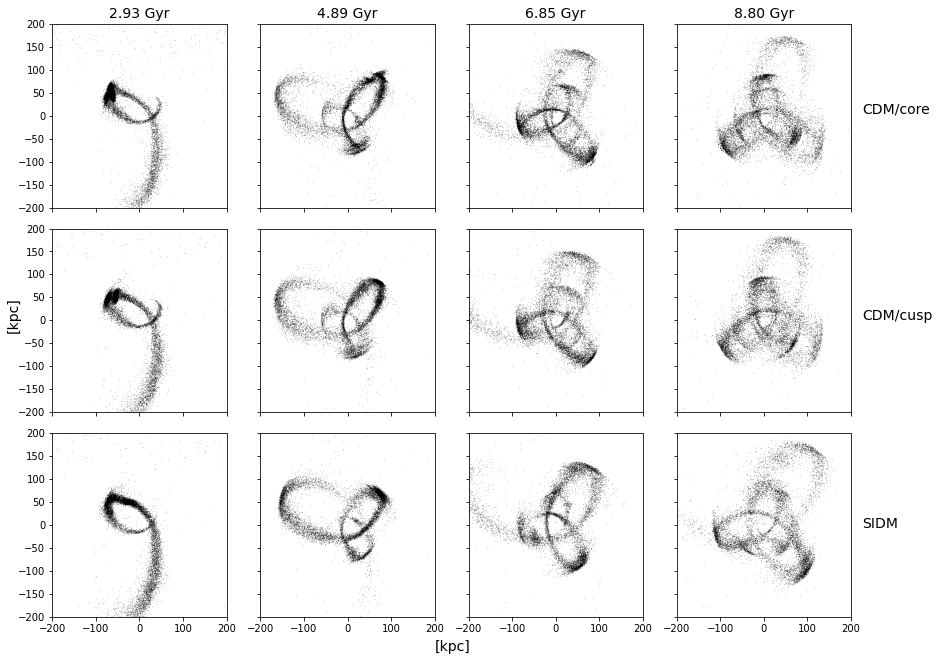
\includegraphics[width=0.9\linewidth]{figs/stars_bw.png}
    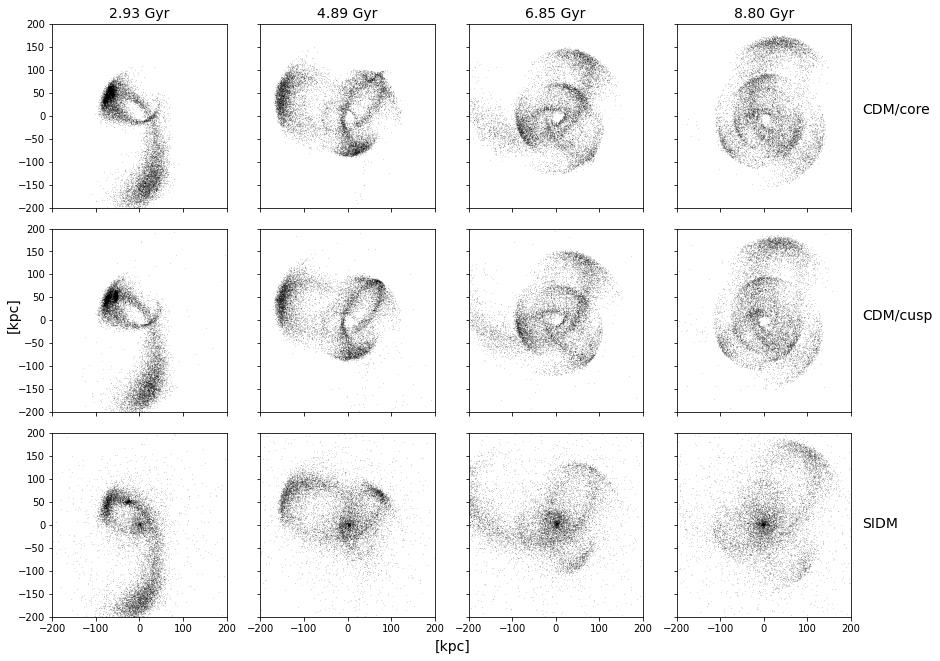
\includegraphics[width=0.9\linewidth]{figs/darks_bw.png}
    \caption{%
        Positions of Sgr stellar (top three rows) and dark matter (bottom
        three rows) particles at various times for all three of the considered
        mergers.  Each column denotes a different time; each row a different
        merger.
    }
    \label{fig:inits}
\end{figure}

Even from these plots, there are some interesting patterns to note. First, we
notice the development of a winding stream structure much like that reported
in~\cite{dierickx_predicted_2017} by around 6 to 7 Gyr in all three cases. We
can also note that the CDM/core and CDM/cusp streams are rather similar, with
the general shape, size, and overall rotation in agreement. There do exist some
differences particularly at later times, however, particular in the inner
stellar structure. For example, at 6.85 Gyr, one can see a sharply defined inner
stream at $(20,60)$ kpc which is significantly fuzzier and less dense in the
CDM/cusp case. Similar differences emerge at the later 8.80 Gyr time stamp.

There are much more marked differences between the SIDM and CDM cases,
however.  The stream arms appear to be slightly rotated clockwise relative to
the CDM mergers, and the general shape of the inner structure is very
different.  In particular, the CDM merger appear to show doubled-stream shape
for the inner arms at the later time stamps which is entirely non-existent in
the SIDM case.  These differences are even more apparent when looking at the
distribution of dark matter.  In the CDM mergers, the dark matter distribution
appears to roughly trace out the distribution of the stream and has a distinct
hole at the origin.  In the SIDM merger, however, the dark matter distribution
largely loses the precise shape of the stream, instead collapsing inward
toward the MW center.

We can also look at the density of particles in the orbital plane by performing
a two-dimensional histogram on the data in Figure~\ref{fig:inits}.  The result
is shown in Figure~\ref{fig:densities}.  The densities are integrated over the
axis perpendicular to the orbital plane.

\begin{figure}
    \centering
    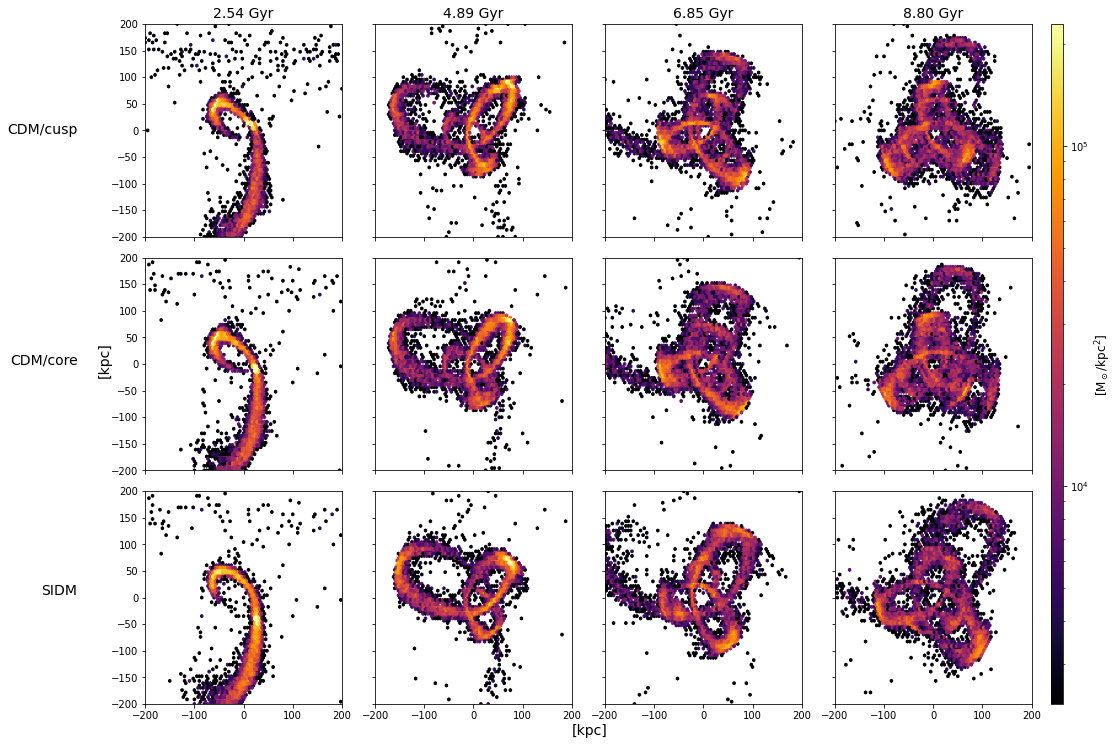
\includegraphics[width=0.9\linewidth]{figs/density_stars.png}
    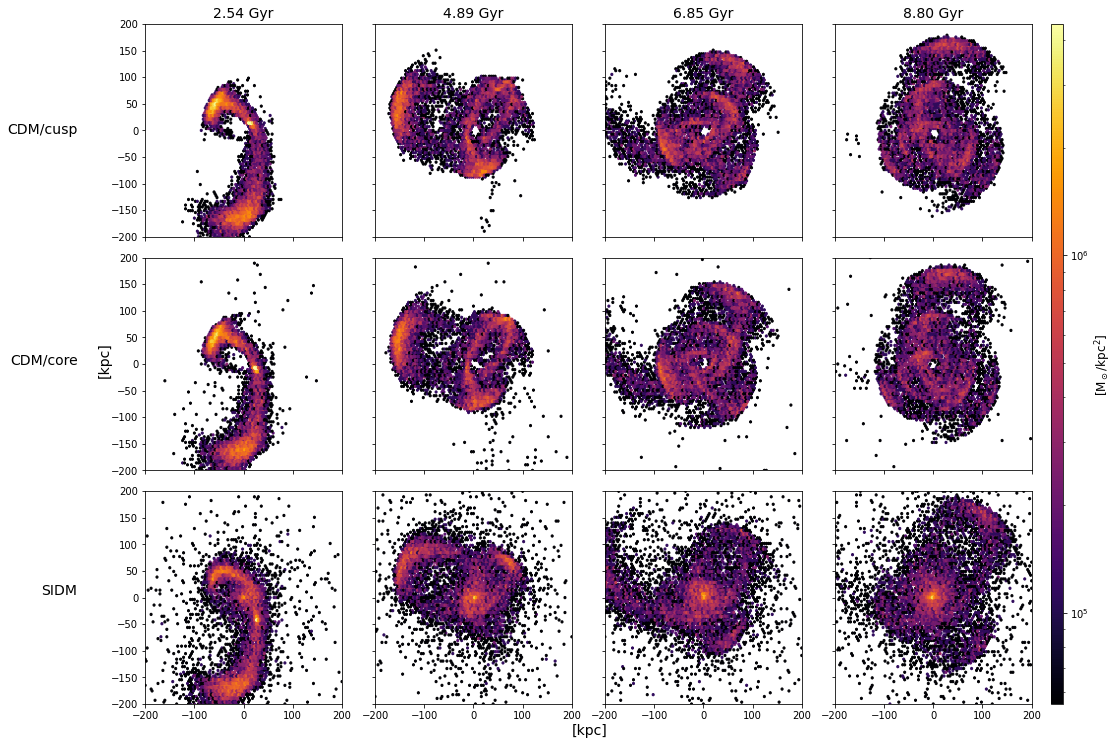
\includegraphics[width=0.9\linewidth]{figs/density_darks.png}
    \caption{%
        Two-dimensional density histogram of the stellar (top three rows) and
        dark matter (bottom three rows) Sgr particles at various times for
        each considered merger.  Densities are integrated over the axis
        perpendicular to the orbital plane.
    }
    \label{fig:densities}
\end{figure}

The density plots allow us to more strictly quantify some of the trends noted
previously. For example, the dark matter density plots show quite concretely
that the dark matter distribution in the SIDM case peaks at the Galactic center,
where there is a distinct hole in the CDM mergers. The SIDM particles are also
significantly less well-constrained, with a large spread extending beyond the
limits of the plot. This is compared to the CDM cases, where there are
relatively few particles outside of the path of the stream.

Looking at the density distribution of the stellar particles allows us to
quantify some of the differences noted earlier.  For example, at 6.85 Gyr, the
SIDM stream has a relatively high-density ($\sim 10^5$ M$_\odot$/kpc$^2$)
stream arc extending from approximately $(-20,0)$ kpc up to around $(60,125)$
kpc.  The corresponding arc exists in the CDM cases, but it is less
well-defined (there is more horizontal spread) and lower density ($\sim 10^4$
M$_\odot$/kpc$^2$).

There are other, similar differences, but we would do better to analyze these
differences for the specific time stamps of each merger which most closely
approximate Sgr today. Determining this requires mapping the position of the Sgr
progenitor, however.


\hypertarget{identifying-the-sgr-progenitor}{%
\section{Identifying the Sgr
progenitor}\label{identifying-the-sgr-progenitor}}

A key part of analyzing these data is to understand the trajectory and
evolution of the Sgr progenitor.  As such, we desire a method for successfully
identifying the position of the Sgr progenitor throughout its evolution.  This
is less straightforward than it may sound because of the strong effects of
tidal stripping.  These mean that we need to identify which particles are
stripped or bound to the progenitor at any given point and omit stripped
particles from our calculation of the progenitor position.  In our tests, we
tried a few different methods which we will describe here.

The first method that we tried was to track bound versus unbound star
particles by counting particles as stripped once they exceeded a fixed radius
from the center of mass of bound particles.  The algorithm for this is as
follows.  We begin by counting the stellar particles within a certain radius
on the first snapshot to be ``bound''.  For each snapshot after, we find the
center of mass of the bound particles.  Then, for each bound particle, we
compute its distance from the center of mass.  If this exceeds the fixed
stripping radius, we unmark the star as bound and continue.

As stated, this algorithm has two parameters that can be tuned: the initial
stripping radius for the initial Sgr stellar positions and the fixed stripping
radius for all following snapshots.  We found it useful to describe the
initial stripping radius instead in terms of the percentage of particles that
are initially counted as ``bound''.  For example, we say that the we start
with the innermost 20\% of particles and proceed with a fixed radius of 20
kpc.  The results of applying this algorithm to the CDM/cusp merger data with
a few different choices of parameters can be seen in
Figure~\ref{fig:fixed_star}.

\begin{figure}
    \centering
    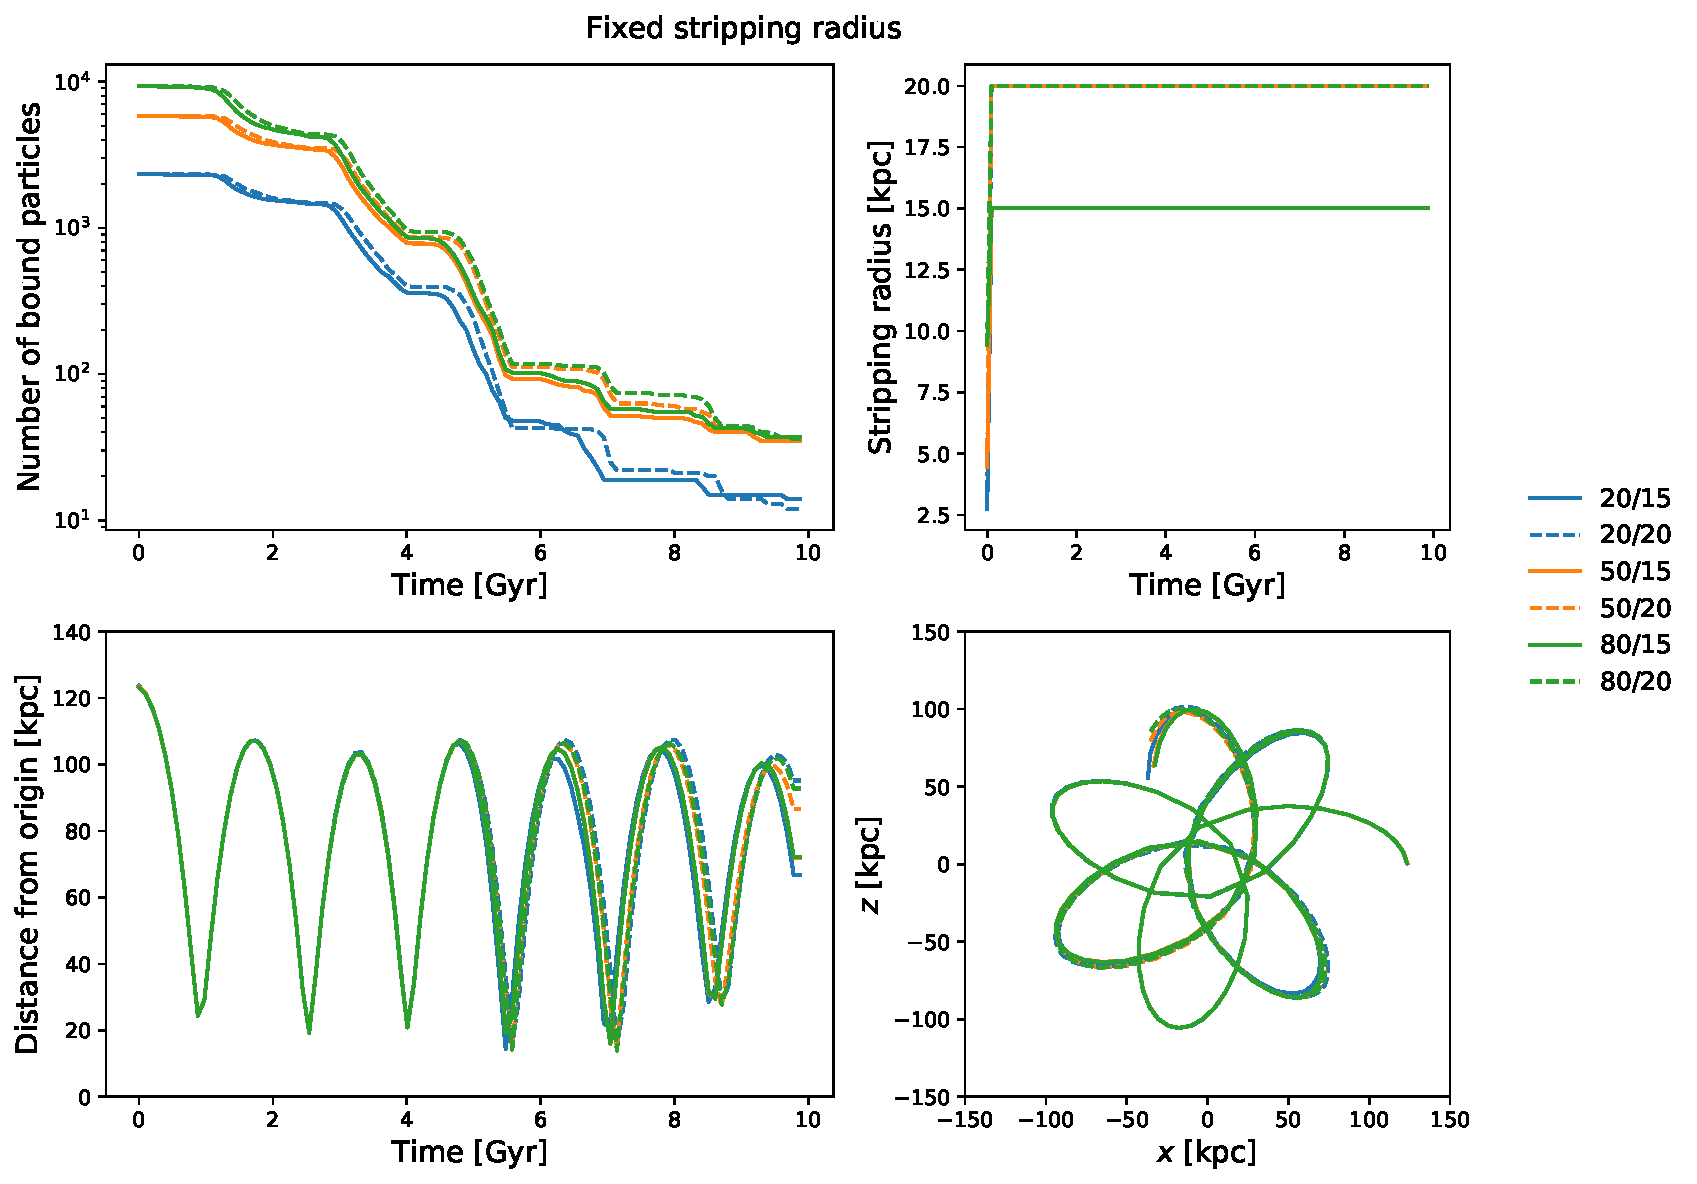
\includegraphics[width=0.9\linewidth]{figs/fixed_star.pdf}
    \caption{%
        Results of applying the ``fixed stripping radius''
        progenitor-identifying algorithm to the CDM/cusp merger data. Entries in
        the legend are given in the following format: ``a/b'' means that we
        started with the innermost ``a''\% of stellar particles and proceeded
        with a fixed stripping radius of ``b'' kpc.  In the upper left is the
        number of bound particles over time.  The upper right shows the
        stripping radius.  The bottom left shows the distance from the origin
        to the Sgr center of mass; an estimate of the MW-Sgr separation.  The
        bottom right shows the trajectory of the progenitor in the orbital
        plane.
    }
    \label{fig:fixed_star}
\end{figure}

This figure shows us that starting with too few of the initial particles (in
this case, 20\%) leads to very small numbers of bound particles at late times.
Further, it shows us that the trajectory of the progenitor can be somewhat
sensitive to the chosen algorithm parameters, especially at late times.

This algorithm appears to have two issues that we want to try to solve.
First, the actual size of the progenitor is expected to shrink with time, as
progressively more of the particles are stripped.  By using a fixed stripping
radius, we are not modeling the expected decay of the progenitor size.  The
second problem we encountered is that this method appears to leave us with
only $\mathcal{O}(10)$ bound particles after around 6 Gyr evolved.  As such,
we decided to explore modifications to the algorithm.

The first modification was to consider a decreasing stripping radius.  The
algorithm is very similar to before.  On the first snapshot, we count some
inner fraction of the particles to be ``bound'' and find the radius of this
ball of bound particles.  For the next snapshot, we strip any particles
which exceed this radius (times a constant).  \textit{However}, after
stripping away particles, we recompute the radius of the ball of the bound
particles, and reset the stripping radius equal to this. For each snapshot
following, we strip particles that are beyond this radius and recompute the
radius.  Over time, the stripping radius will decrease, modeling the
progressively decreasing size of the progenitor.  Some basic tests showed that
this algorithm often becomes a bit too aggressive, so we introduced a minimum
stripping radius, such that the algorithm would never use too small a stripping
radius. 

Further testing with a minimum stripping radius of 8 kpc and a variety of
different initial parameters showed the algorithm to simply be too aggressive.
For all considered combinations of parameters, we found that the algorithm
reduced itself below the minimum stripping radius by around 6 Gyr.  This means
that at later times, when we might expect the closest resemblance to the
observed Sgr progenitor, the algorithm reduces to the fixed stripping radius
algorithm with a fixed radius of 8 kpc. 

One possible reason that it becomes too aggressive is because the actual
size of the progenitor is not monitonically decreasing.  Rather, its size
fluctuates over the course of the orbit, becoming quite compressed and small
near the pericenter and a bit more spread out and large near the apocenter.
These effects are modeled by the King formula for the tidal
radius~\cite{king_structure_1962} as given in~\cite{dierickx_predicted_2017}:
\begin{equation} \label{eq:king_radius}
    r_t = r \left[ \frac{1}{2} 
    \frac{M_{\text{Sgr}}(<r_t)}{M_{\text{MW}}(<r)} \right]^{1/3},
\end{equation}
where $M_{\text{gal}}(<r)$ is the enclosed halo mass in galaxy ``gal'' within
radius $r$ of the center of mass of the galaxy, $r$ is the distance between
the Milky Way and Sgr centers of mass, and $r_t$ is the tidal radius.  For a
given snapshot, then, we can compute the tidal radius according to this
formula by subtracting $r_t$ from both sides and using a simple root finder to
identify the $r_t$ which solves the equation.  We then strip any particles
which are farther than $r_t$ away from the center of mass of the progenitor at
the current time.  Again, initial testing showed that this algorithm needed a
minimum stripping radius to prevent it from stripping away all the stellar
particles.

Further testing with a minimum stripping radius of 8 kpc showed this algorithm
to also be too aggressive.  We tried to add a multiplicative factor to the tidal
radius in order to make it a little larger before stripping, but this did not
appear to help very much. After only a few Gyr, this too reduced effectively to
the fixed radius strategy, using only the minimum stripping radius.

At this point, we concluded that the issue of too few bound particles at late
times may be a problem related to our relatively small number of Sgr stellar
particles, instead of a problem with the algorithms themselves.  As such, we
decided to try to use the fixed radius algorithm but using both stellar
\textit{and} dark matter particles.  The result on the CDM/cusp data is shown
in Figure~\ref{fig:fixed_both}.

\begin{figure}
    \centering
    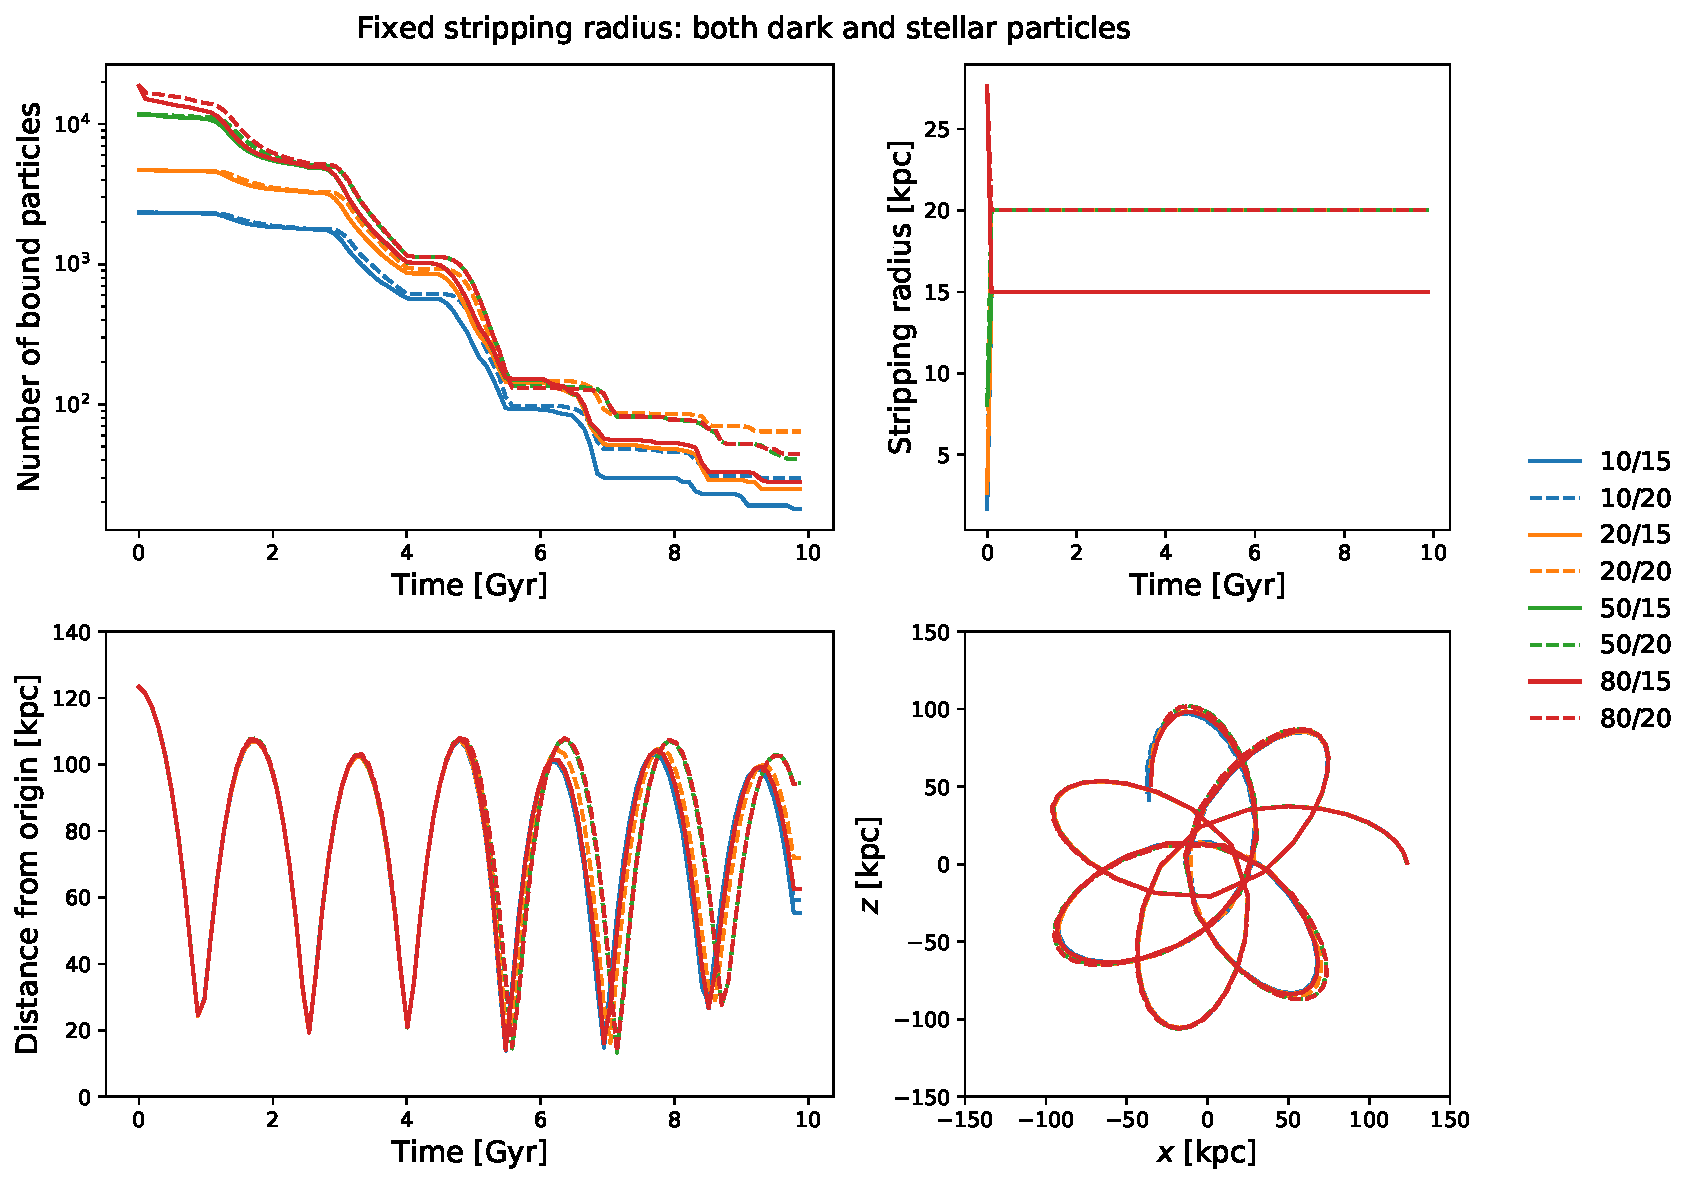
\includegraphics[width=0.9\linewidth]{figs/fixed_both.pdf}
    \caption{%
        Results of using the ``fixed stripping radius'' progenitor-identifying
        algorithm on the all particles in the CDM/cusp merger data. Plots and
        legend entries have the same meaning as in
        Figure~\ref{fig:fixed_star}.
    }
    \label{fig:fixed_both}
\end{figure}

This appears to yield promising results. We note that there are generally more
``bound'' particles at late times when using all particles than when only using
stellar ones, and that, aside from the ``50/20'' and ``80/20'' runs, the
resulting trajectories appear to be more robust to the algorithm parameters. As
such, we choose to move forward with this algorithm using the ``20/20''
parameters, as they appear to be consistent with the majority of the other
parameter choices and yield the most bound particles in the end. Using these
choices to identify the progenitor, we apply the algorithm to all three mergers.
The resulting data are shown in Figure~\ref{fig:all}.

\begin{figure}
    \centering
    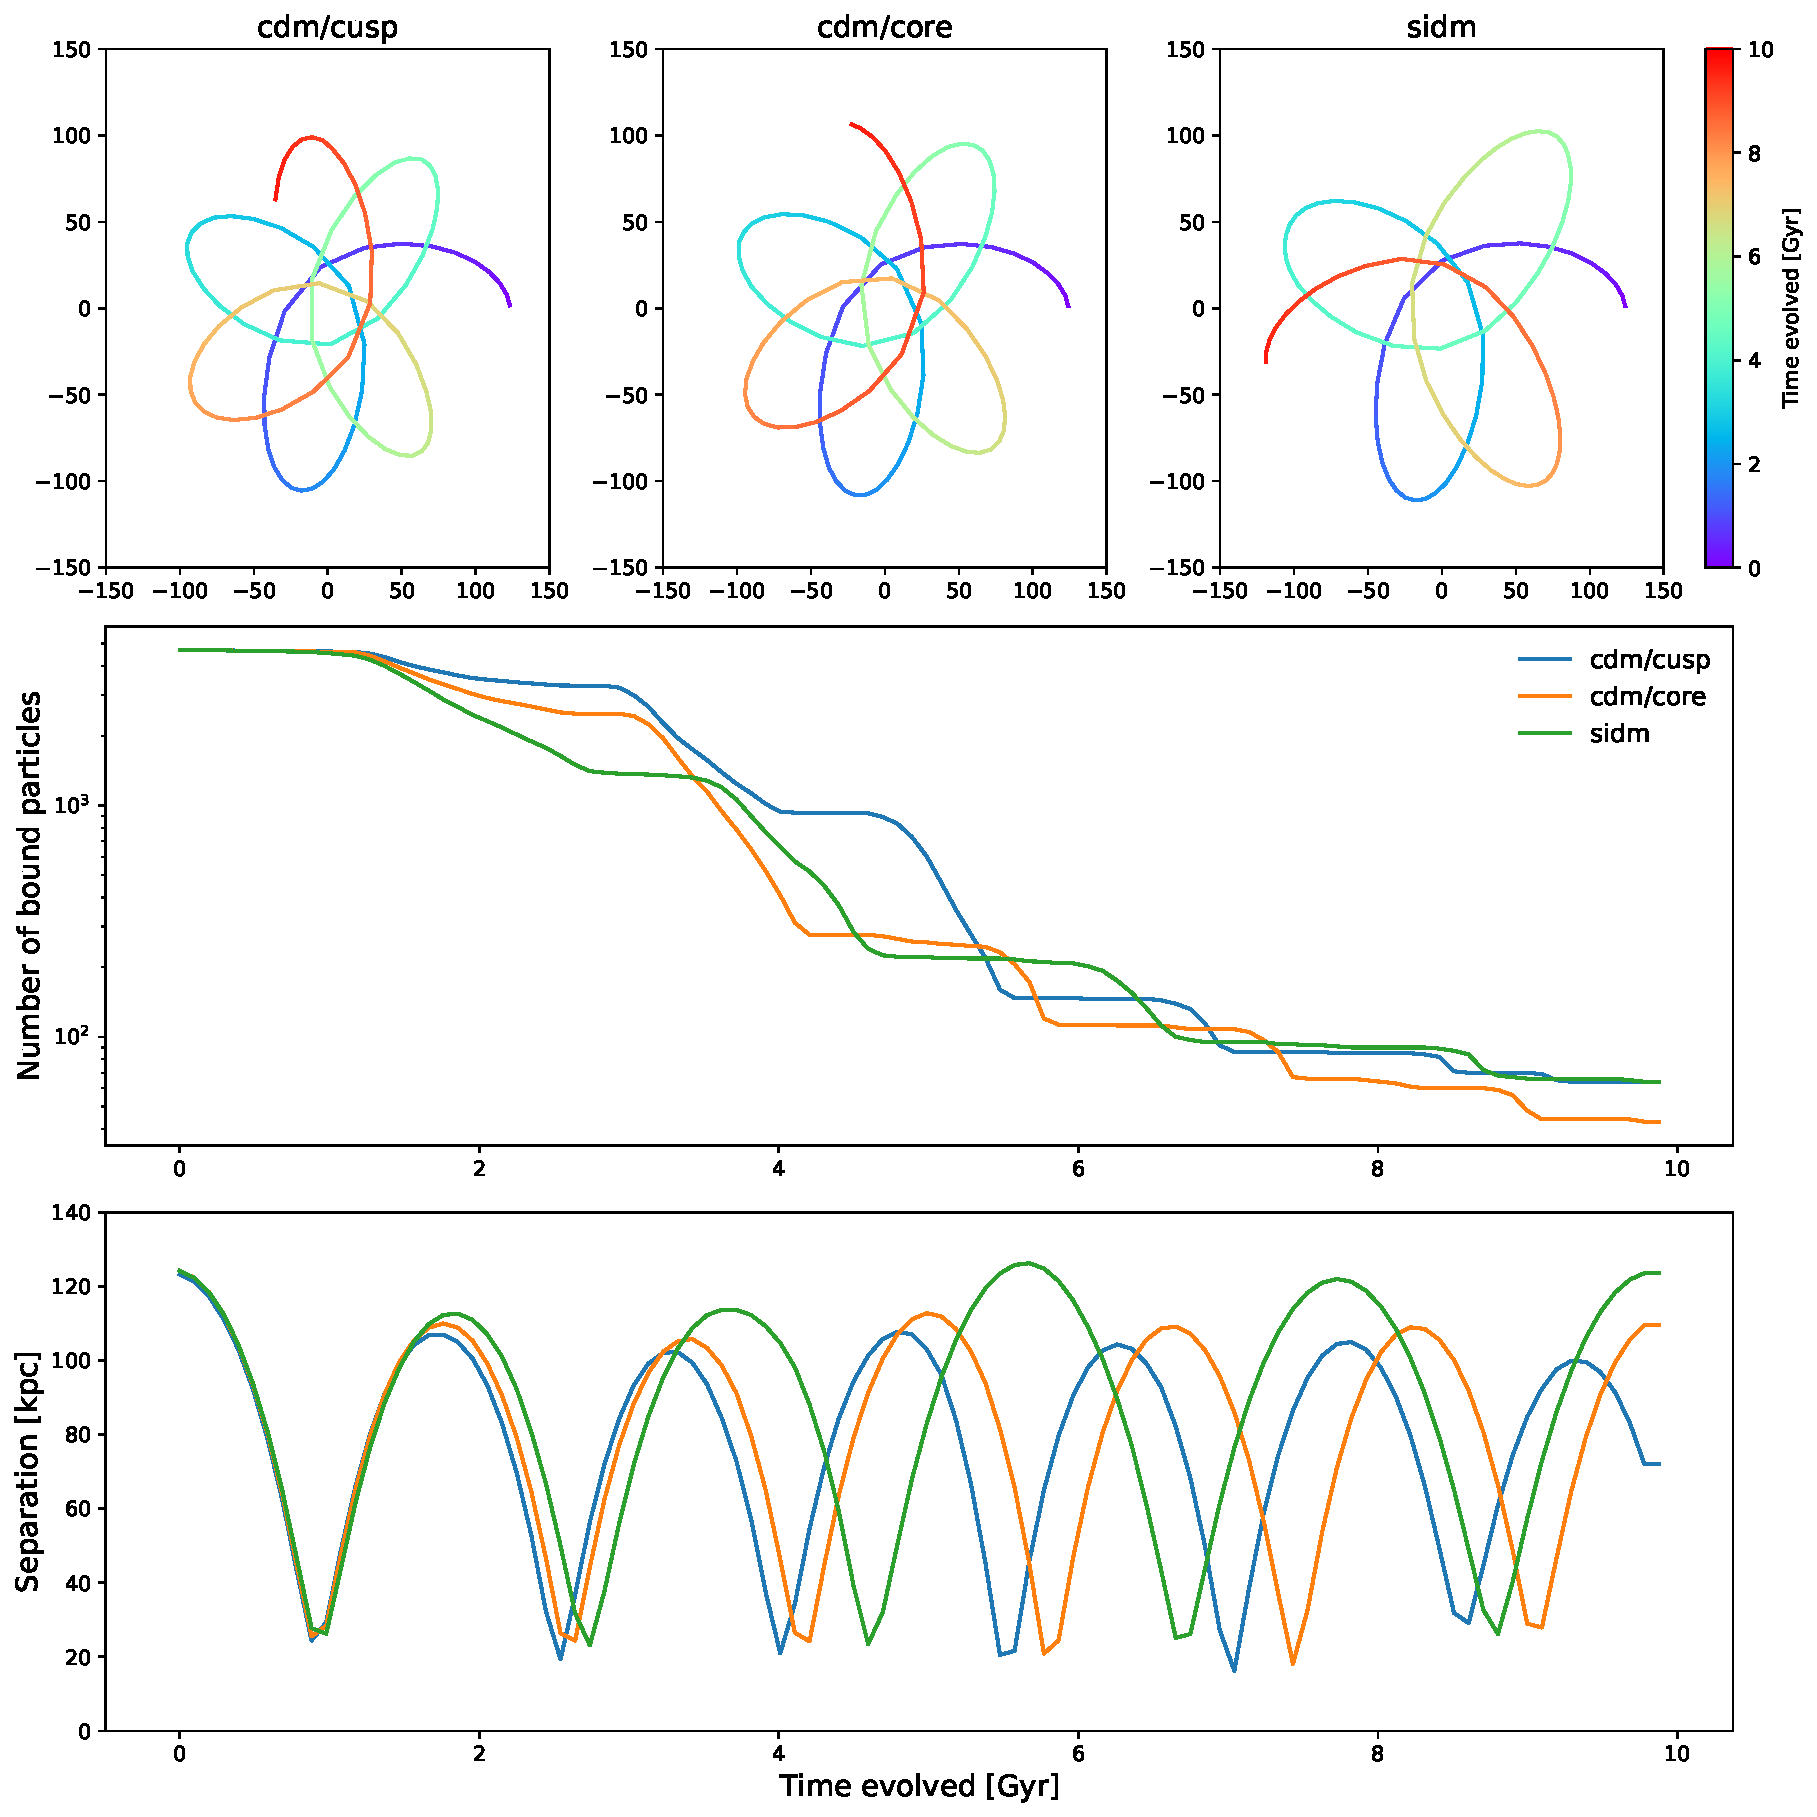
\includegraphics[width=0.9\linewidth]{figs/all_mergers_pretty.pdf}
    \caption{%
        Results of using the ``fixed stripping radius'' progenitor-identifying
        algorithm on all the particles in each of the mergers. We use the
        ``20/20'' algorithm parameters for all mergers, meaning that we start
        with the inner 20\% of particles and use a 20 kpc stripping radius. The
        top row shows the trajectory of the Sgr progenitor in the orbital plane
        for each merger. The middle row plot shows the number of bound particles
        over time. The bottom row plot shows the MW-Sgr separation over time.
    }
    \label{fig:all}
\end{figure}

The plots in this figure are evidence that SIDM microphysics may indeed have a
profound impact on the resulting trajectory of the Sgr satellite.  One such
difference is that the number of bound particles decreases much more
substantially at early times than either of the two CDM runs.  This could be
explained by considering that self-interactions provide a mechanism for dark
matter to free itself from shallow gravitational potential wells to which
collisionless dark matter would remain confined.

Looking at the MW-Sgr separation over time, it is immediately evident that the
cored profile yields a slightly longer orbital period, given the slowly
increasing distance between the apo- and pericenters of the CDM/cusp and
CDM/core orbits.  The inclusion of self-interactions appears to add to this
effect, with the CDM/cusp progenitor attaining six pericenters before the SIDM
orbit is able to reach a fifth.

One phenomenon showcased by the separation curves which is difficult to
understand is the lack of a consistent decay in the apocenters.  We compare to
Figure 6 of~\cite{dierickx_predicted_2017}, which shows a steadily decreasing
apocenter.  This is the expected behavior; as the Sgr progenitor orbits and
decays, we would expect it to lose energy and steadily fall inward.  This,
however, does not appear in our plots.  In fact, this phenomenon is
exacerbated in the SIDM merger, where the apocenter actually appears to
\textit{grow} after around 4 Gyr, reaching nearly 130 kpc at the 6 Gyr mark.
The mechanism by which this would occur is not yet understood.

Future studies would do well to explore other algorithms for identifying the Sgr
progenitor, such as a friends-of-friends (FOF) halo-finder. These difficulties
would also likely be alleviated by greater stellar resolution through the use of
more stellar particles and the inclusion of a stellar bulge. 


% \hypertarget{time-of-closest-match}{%
% \section{Time of closest match}\label{time-of-closest-match}}
\hypertarget{comparison-to-stream-data}{%
\section{Comparison to stream data}\label{comparison-to-stream-data}}

\hypertarget{progenitor-coordinates}{%
\subsection{Progenitor coordinates}\label{progenitor-coordinates}}

As stated previously, a description of the orbit of the progenitor will allow us
to determine the specific time stamps at which our mergers most closely
approximate Sgr today.  We take the observed coordinates of Sgr to be
$(\alpha, \delta) = (283.83, -29.45)$ degrees (where $\alpha$ is right
ascension and $\delta$ is declination)~\cite{nasa_nasaipac_nodate}, proper
motion $(\mu_\alpha \cos\delta, \mu_\delta) = (-2.54 \pm 0.18, -1.19 \pm
0.16)$ mas/yr~\cite{massari_hubble_2013}, heliocentric distance $24.8 \pm 0.8$
kpc~\cite{kunder_distance_2009}, and line-of-sight velocity $179 \pm 1$
km/s~\cite{dierickx_predicted_2017,bellazzini_nucleus_2008}.  

To compare our data to these coordinates, we must convert from Galactocentric
distances in the orbital plane to equatorial coordinates.  We do this using the
Astropy package~\cite{astropy_collaboration_astropy_2013,
astropy_collaboration_astropy_2018} with the assumptions that the Sun is
located at approximately $(8,0,0)$ kpc with a velocity which is approximately
directed in the positive $y$ direction.  The resulting coordinates over time
are shown in Figure~\ref{fig:eq_prog}.  We note that the right ascension data
generally moves from left to right across the plot and is meant to be
interpreted as wrapping around from the right edge back to the left.

\begin{figure}
    \centering
    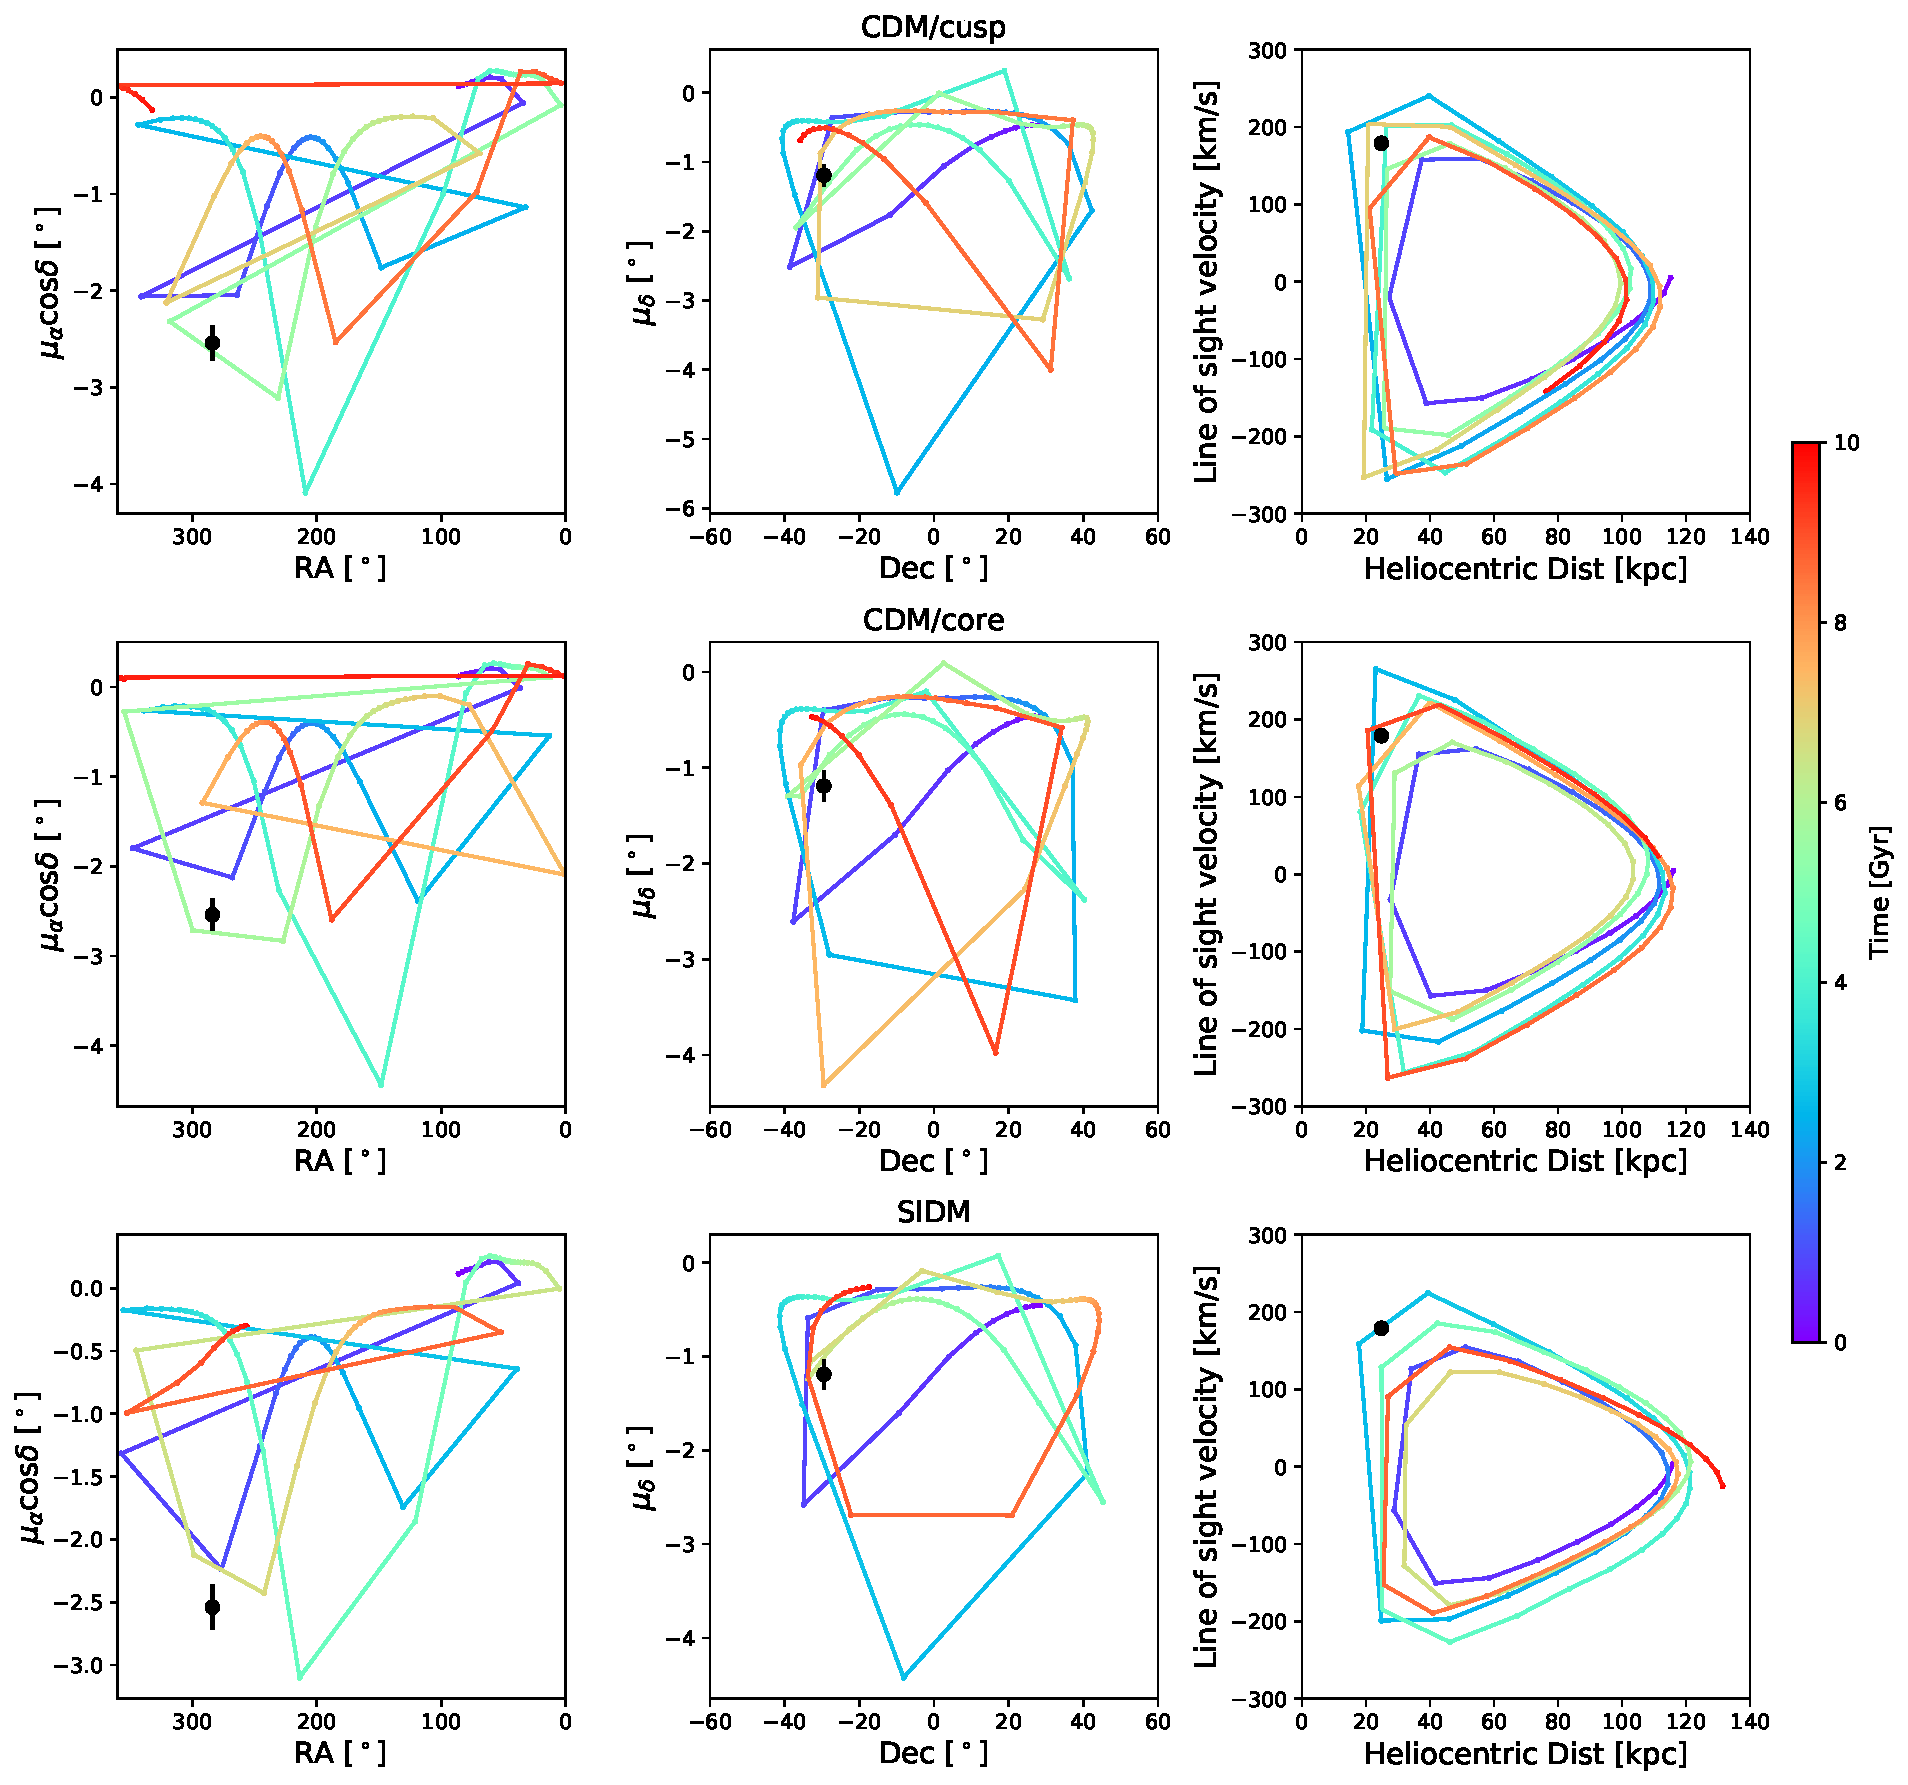
\includegraphics[width=1.0\linewidth]{figs/equatorial_progenitor.pdf}
    \caption{%
        Trajectory of the Sgr progenitor in terms of equatorial coordinates and
        proper motions for each merger. Black squares represent the observed
        coordinates of the progenitor today. Error bars are present for observed
        quantities with uncertainties, though are in some cases smaller than
        the size of the marker (particularly in the velocity versus distance
        subplots).
    }
    \label{fig:eq_prog}
\end{figure}

We note that the Dierickx 2017 model~\cite{dierickx_predicted_2017} most
closely approximated the observed coordinates just after its fifth pericenter,
with the best agreement with the stream shape occurring then as well.
Unfortunately, no snapshot of our model comes as close to these coordinates as
theirs, but we believe that this discrepancy would be alleviated somewhat by
greater time resolution in the snapshots of the stream.  We do, however, find
that the CDM mergers attain their closest matches to the observed coordinates
just after their fifth pericenters (approximately 7.04 Gyr and 7.43 Gyr for
the /cusp and /core cases, respectively), in accord with the Dierickx model.
The SIDM merger attains its closest match after its fourth pericenter
(approximately 6.75 Gyr) with its fifth pericenter (approximately 8.80 Gyr)
the next closest match.

In particular, the line-of-sight velocity versus heliocentric distance plots
in the Figure show a curious trend.  In the CDM cases, the trajectory passes
roughly through the observed velocity and distance with every pericentric
passage except the first.  By contrast, no time stamp of the SIDM merger after
the third pericenter appears to closely replicate the observed velocity.  At
such early times, however, Sgr has not completed enough wraps for the resulting
stream to match existing models, such as Law 2010 or Dierickx 2017.  We also
note that the orbital period of the SIDM merger was seen to be significantly
longer than that of either CDM merger; we believe this to be consistent with
the smaller line-of-sight velocities observed here.

We can also use our progenitor-identifying algorithm to obtain estimates of the
times at which each stellar particle comes unbound from the progenitor. We can
thus look at the line-of-sight velocity and heliocentric distance for each star
of the mergers at their respective fifth pericenters, colored according to their
stripping time. We choose to use the fifth pericenter for the SIDM merger as
well because it gives the best agreement with the observed distance and
line-of-sight velocity at late times, despite poorer agreement with the other
dimensions.  This is shown in Figure~\ref{fig:vel_v_dist}.

\begin{figure}
    \centering
    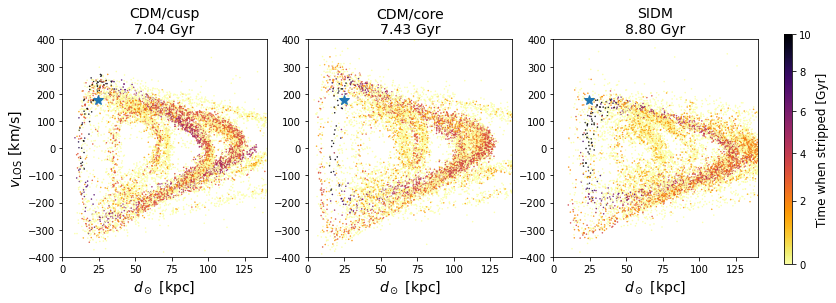
\includegraphics[width=1.0\linewidth]{figs/vel_v_dist_peri_only.png}
    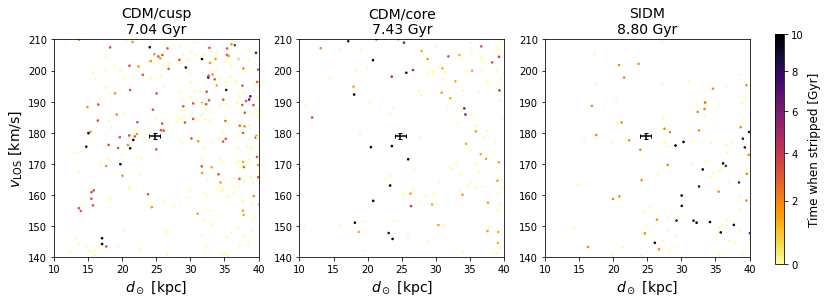
\includegraphics[width=1.0\linewidth]{figs/vel_v_dist_zoomed.png}
    \caption{%
        Line-of-sight velocity versus heliocentric distance for Sgr stellar
        particles in each merger, colored according to the time at which each
        particle became unbound from the progenitor. Each merger is given at its
        fifth pericenter. (Top) The full spread of Sgr stellar particles closer
        than 140 kpc, with the observed coordinates shown as a blue star.
        (Bottom) Only the Sgr stellar particles which are close to the observed
        coordinates; observed coordinates denoted by black error bars.
    }
    \label{fig:vel_v_dist}
\end{figure}

The resulting Figure gives a strong indication that the SIDM stream is indeed
unable to adequately reproduce the observed line-of-sight velocity of Sgr. In
particular, we note that both CDM mergers display a number of bound (colored
dark) particles which roughly surround the observed coordinates.  The SIDM
merger, however, shows that all bound particles either have too small a
line-of-sight velocity or too large a heliocentric distance to yield the
observed progenitor coordinates. We note further that this discrepancy is very
significant with respect to the uncertainties in the measured coordinates.

% \hypertarget{comparison-to-stream-data}{%
% \section{Comparison to stream data}\label{comparison-to-stream-data}}

\hypertarget{stream-shape}{%
\subsection{Stream shape}\label{stream-shape}}

The next piece of the analysis that we will consider is a comparison to data
from the second data release (DR2) of the \textit{Gaia}
mission~\cite{lindegren_gaia_2018,gaia_collaboration_gaia_2018}, from which Sgr
stars have been identified by Ibata et al.~\cite{ibata_panoramic_2020} using the
\verb|STREAMFINDER| (hereafter \verb|SF|)
algorithm~\cite{malhan_streamfinder_2018, malhan_ghostly_2018}.  The resulting
dataset includes the \textit{Gaia} equatorial coordinates, proper motions,
magnitudes, and colors of 263,438 stars, along with an estimate of the
distance provided by the algorithm.  They find their dataset to agree well
with the Law 2010 model~\cite{law_sagittarius_2010}, barring a few small
deviations.  The \verb|SF| sample is shown in equatorial coordinates in
Figure~\ref{fig:streamfinder}.  We note in particular a very dense region of
stars at around $\alpha = 280^\circ$, $\delta = -30^\circ$, and heliocentric
distance $\approx 30$ kpc.  This is the Sagittarius progenitor.

\begin{figure}
    \centering 
    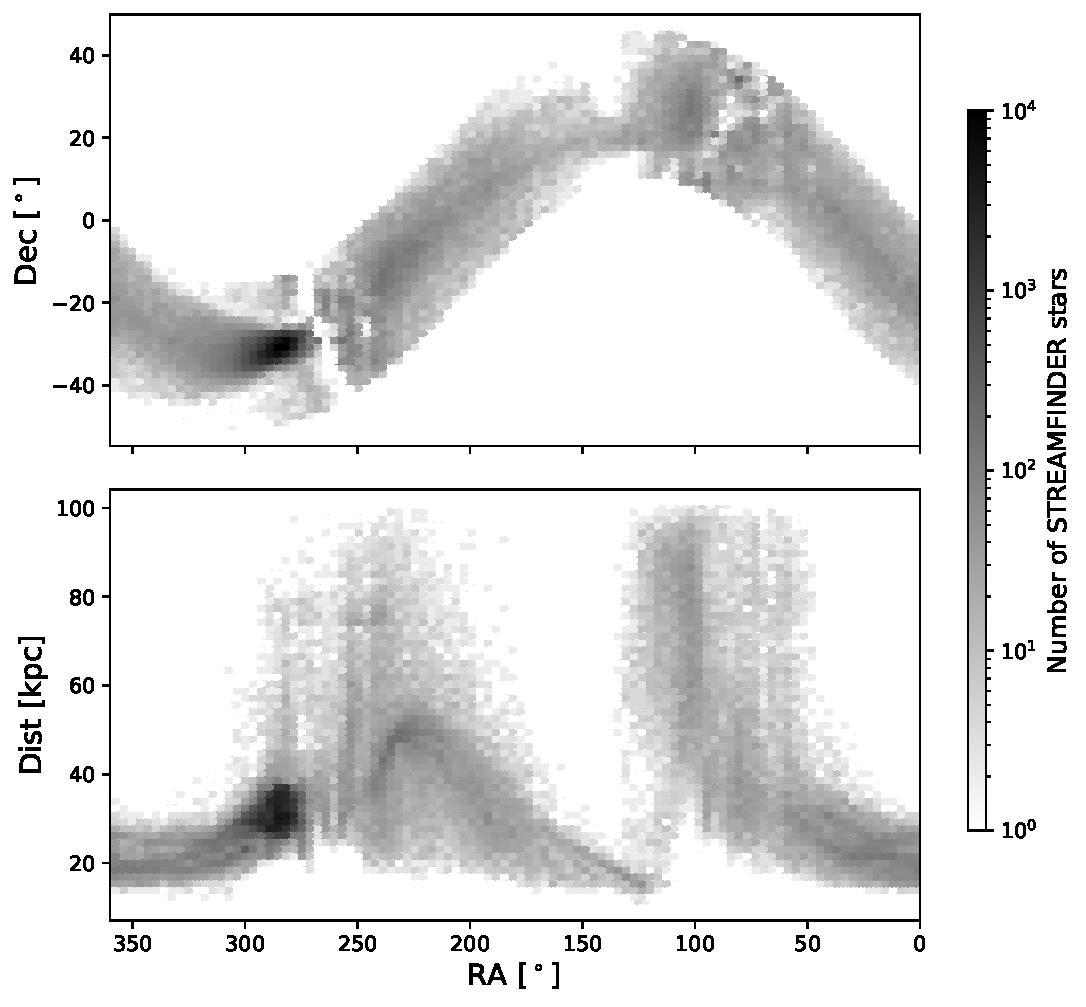
\includegraphics[width=0.7\linewidth]{figs/streamfinder.pdf}
    \caption{%
        Equatorial coordinates and estimated heliocentric distances for the
        263,438 Sgr stars identified by the \texttt{STREAMFINDER} algorithm.
    }
    \label{fig:streamfinder}
\end{figure}

For each merger, we continue to consider the fifth pericenter as before. We
again convert to equatorial coordinates, this time using only those stars with a
heliocentric distance less than 100 kpc, as the \verb|SF| sample
contains no stars beyond this threshold. The resulting distribution of stars is
plotted in Figure~\ref{fig:equatorial} with the \verb|SF| density
shown in gray.

\begin{figure}
    \centering 
    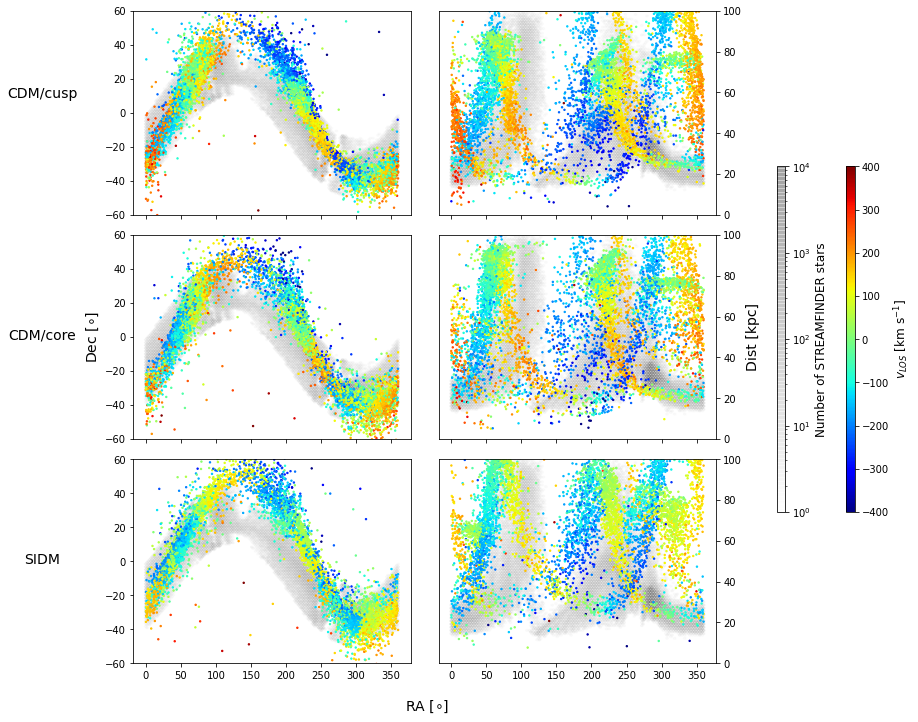
\includegraphics[width=1.0\linewidth]{figs/equatorial_streamfinder.png}
    \caption{%
        Equatorial coordinates for our simulated Sgr stellar particles of
        distances less than 100 kpc at the time of the fifth pericenter for
        each mergeri, colored by line-of-sight velocity.  The position of the
        simulated progenitor is shown by a white circle with black outline.
        (Note that it is located at RA $\approx 0.5^\circ$ in the CDM/core
        plots.) The observed coordinates of Sgr are shown as a black circle.
        The density of \texttt{STREAMFINDER} stars is shown in gray.
    }
    \label{fig:equatorial}
\end{figure}

Our comparison to the \verb|SF| stars shows qualitatively good agreement in
terms of the right ascension and declination, as the simulated streams appear
to reach their maximum and minimum values of declination at the same right
ascensions as the \verb|SF| stream.  We note that our streams are less thick
in most areas, perhaps owing to a smaller number of stellar particles.  Our
streams also reach a greater maximum declination than the \verb|SF| data; this
discrepancy appears to impact the CDM/cusp merger the least and the SIDM
merger the most.  The SIDM merger in general appears to have larger
declination values than expected from data.

When looking at the distribution of heliocentric distances, we note relatively
good agreement for right ascensions larger than $200^\circ$ in the CDM cases.
For smaller right ascensions, we do see the reproduction of the stream arm, but
shifted slightly toward larger right ascensions. This effect appears to be
less present in the CDM/core case. The SIDM merger also appears to reproduce the
stream arm for smaller right ascension, but is substantially less accurate at
reproducing that of larger right ascensions, with the whole of the stream
appearing to be shifted up by roughly $60^\circ$. The heliocentric distance
distribution also shows the predicted extensions to the leading and trailing
stream arms from the Dierickx model. 

When plotted in these coordinates, we can also discern some differences between
the mergers themselves. As an example, we can again see a marked difference in
the distribution of line-of-sight velocities, as the CDM mergers both show a
rather significant number of stars with large, positive line-of-sight
velocities (in the orange-red region of the colormap). The SIDM merger, by
contrast, has very few such stars, preferring smaller velocities. Unfortunately,
the \verb|SF| dataset does not come with radial velocities; as such, we choose
to use another dataset for this comparison.


\hypertarget{twomass}{\subsection{2MASS M-giants}\label{twomass}}

The final comparison we will make is with M-giant stars from the Two Micron All
Sky Survey (2MASS) as identified by Majewski et al.~\cite{majewski_two_2003}.
There are significantly fewer stars in this dataset (only 202), but they all
include line-of-sight velocity and heliocentric distance information, allowing
us to directly compare these quantities with our simulated streams. We note
further that these stars explicitly correspond to the leading and trailing arms
of Sgr, not the progenitor.

We begin with a full comparison of our three simulated streams against the 2MASS
data in terms of right ascension, declination, heliocentric distance, and
line-of-sight velocity. The comparison is shown in Figure~\ref{fig:eq_2mass}. 

\begin{figure}
    \centering
    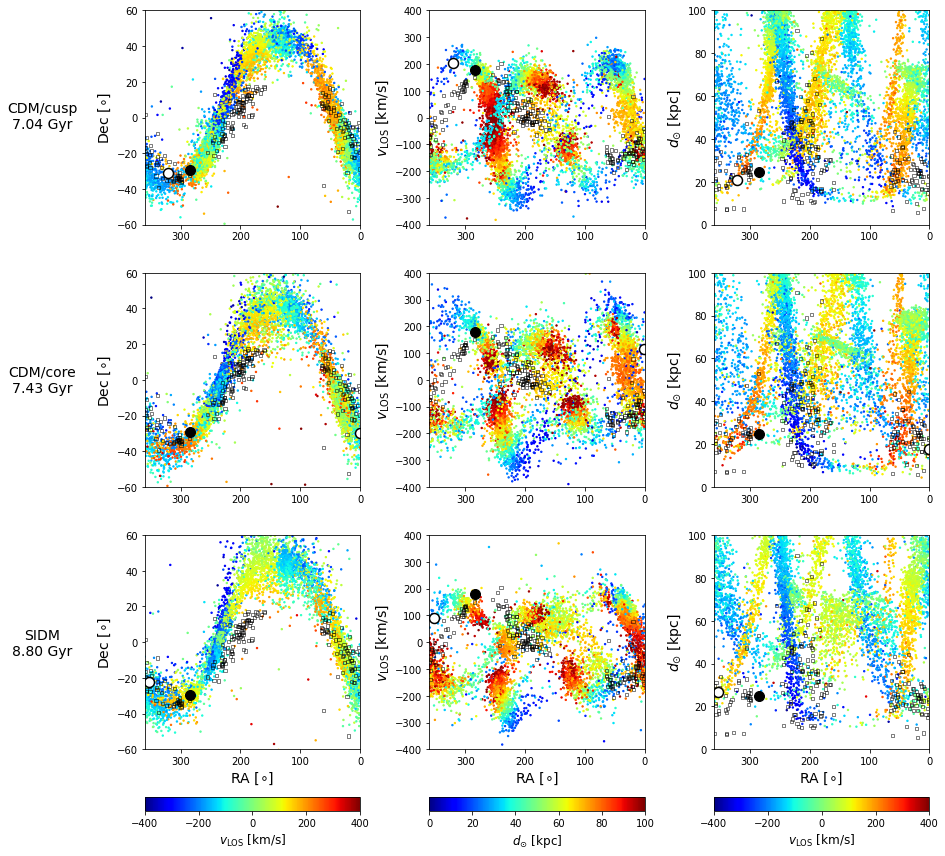
\includegraphics[width=1.0\linewidth]{figs/equatorial_2mass.png}
    \caption{%
        Right ascension, declination, heliocentric distance, and line-of-sight
        velocity for our simulated streams at their fifth pericenters. The white
        circle gives the position of the simulated progenitor; the black circle
        gives the observed coordinates of the progenitor.  The black squares
        correspond to 2MASS M-giant stars, identified by
        Majewski~\cite{majewski_two_2003}.
    }
    \label{fig:eq_2mass}
\end{figure}

This Figure appears to show good agreement especially between our CDM mergers
and the 2MASS data. In particular, the right ascension and declination data are
almost entirely reproduced by the CDM streams, with fairly good agreement in
terms of line-of-sight velocity and heliocentric distance. The SIDM stream,
however, gives a much poorer reproduction of the 2MASS stream. Most prominently,
at right ascensions near $200^\circ$, the corresponding declinations are all
significantly greater than the 2MASS data.

We next compare our data to specifically the heliocentric distances and
line-of-sight velocities by reproducing Figure~\ref{fig:vel_v_dist} with the
2MASS data overlaid. The result is shown in Figure~\ref{fig:vel_v_d_2mass}.

\begin{figure}
    \centering
    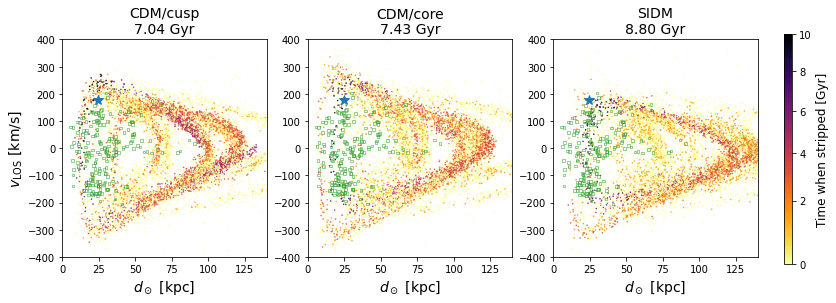
\includegraphics[width=1.0\linewidth]{figs/vel_v_dist_2mass.png}
    \caption{%
        Line-of-sight velocity versus heliocentric distance for each of the
        three mergers at their respective fifth pericenters. The blue star
        denotes the observed distance and velocity; the green squares denote
        data from 2MASS M-giant stars. 
    }
    \label{fig:vel_v_d_2mass}
\end{figure}

This Figure again shows good general agreement between the mergers and the
data.  In particular, the CDM/core merger accurately reproduces many of the
features of the 2MASS data at small heliocentric distances, including the
distances of the closest stars.  The CDM/cusp merger is the next most accurate
in this region, with its closest stars being only a small amount ($\sim 5$
kpc) farther away than given by 2MASS data.  The SIDM merger again has the
worst agreement of the mergers, with very few stars at small heliocentric
distances and low line-of-sight velocities.

These plots give more evidence to believe that the distribution of
line-of-sight velocities in simulations of the Sgr stream can prove to show
important differences between the CDM and SIDM dark matter models. In
particular, we have seen that our CDM models are generally able to reproduce
the Sgr stream more faithfully than can the corresponding SIDM model.

todo round out this thought


% There also exist some differences between the three mergers in this frame.
% For example, the CDM/cusp run appears to have more particles with larger
% line-of-sight velocity magnitudes, with more stars that appear to be dark blue
% and red.  Inversely, the SIDM merger appears to have much more limited
% variation in line-of-sight velocity.  Also, the SIDM and CDM runs appear to
% have different features which are well-defined; the CDM runs show a rising
% stream arm at right ascension $\approx 350^\circ$ that is not well-represented
% in the SIDM run.  The SIDM run, however, has a more well-defined falling
% stream arm at right ascension $\approx 200^\circ$.

% To more fully explore these distances, we can look at histograms of the stellar
% particles' equatorial coordinates and proper motions and compare to the same for
% the \verb|STREAMFINDER| stars. We note, however, the presence of a very dense
% region of stars in the \verb|STREAMFINDER| data at $\text{RA} = 290^\circ$,
% $\text{Dec} = -30^\circ$, and $\text{dist} = 30$ kpc. This greatly skews the
% \verb|STREAMFINDER| distributions, so we cut it off in the plots in order to
% more fully elucidate the simulation distributions. The resulting histograms may
% be seen in Figure~\ref{fig:eq_hists}.

% \begin{figure}
%     \centering
%     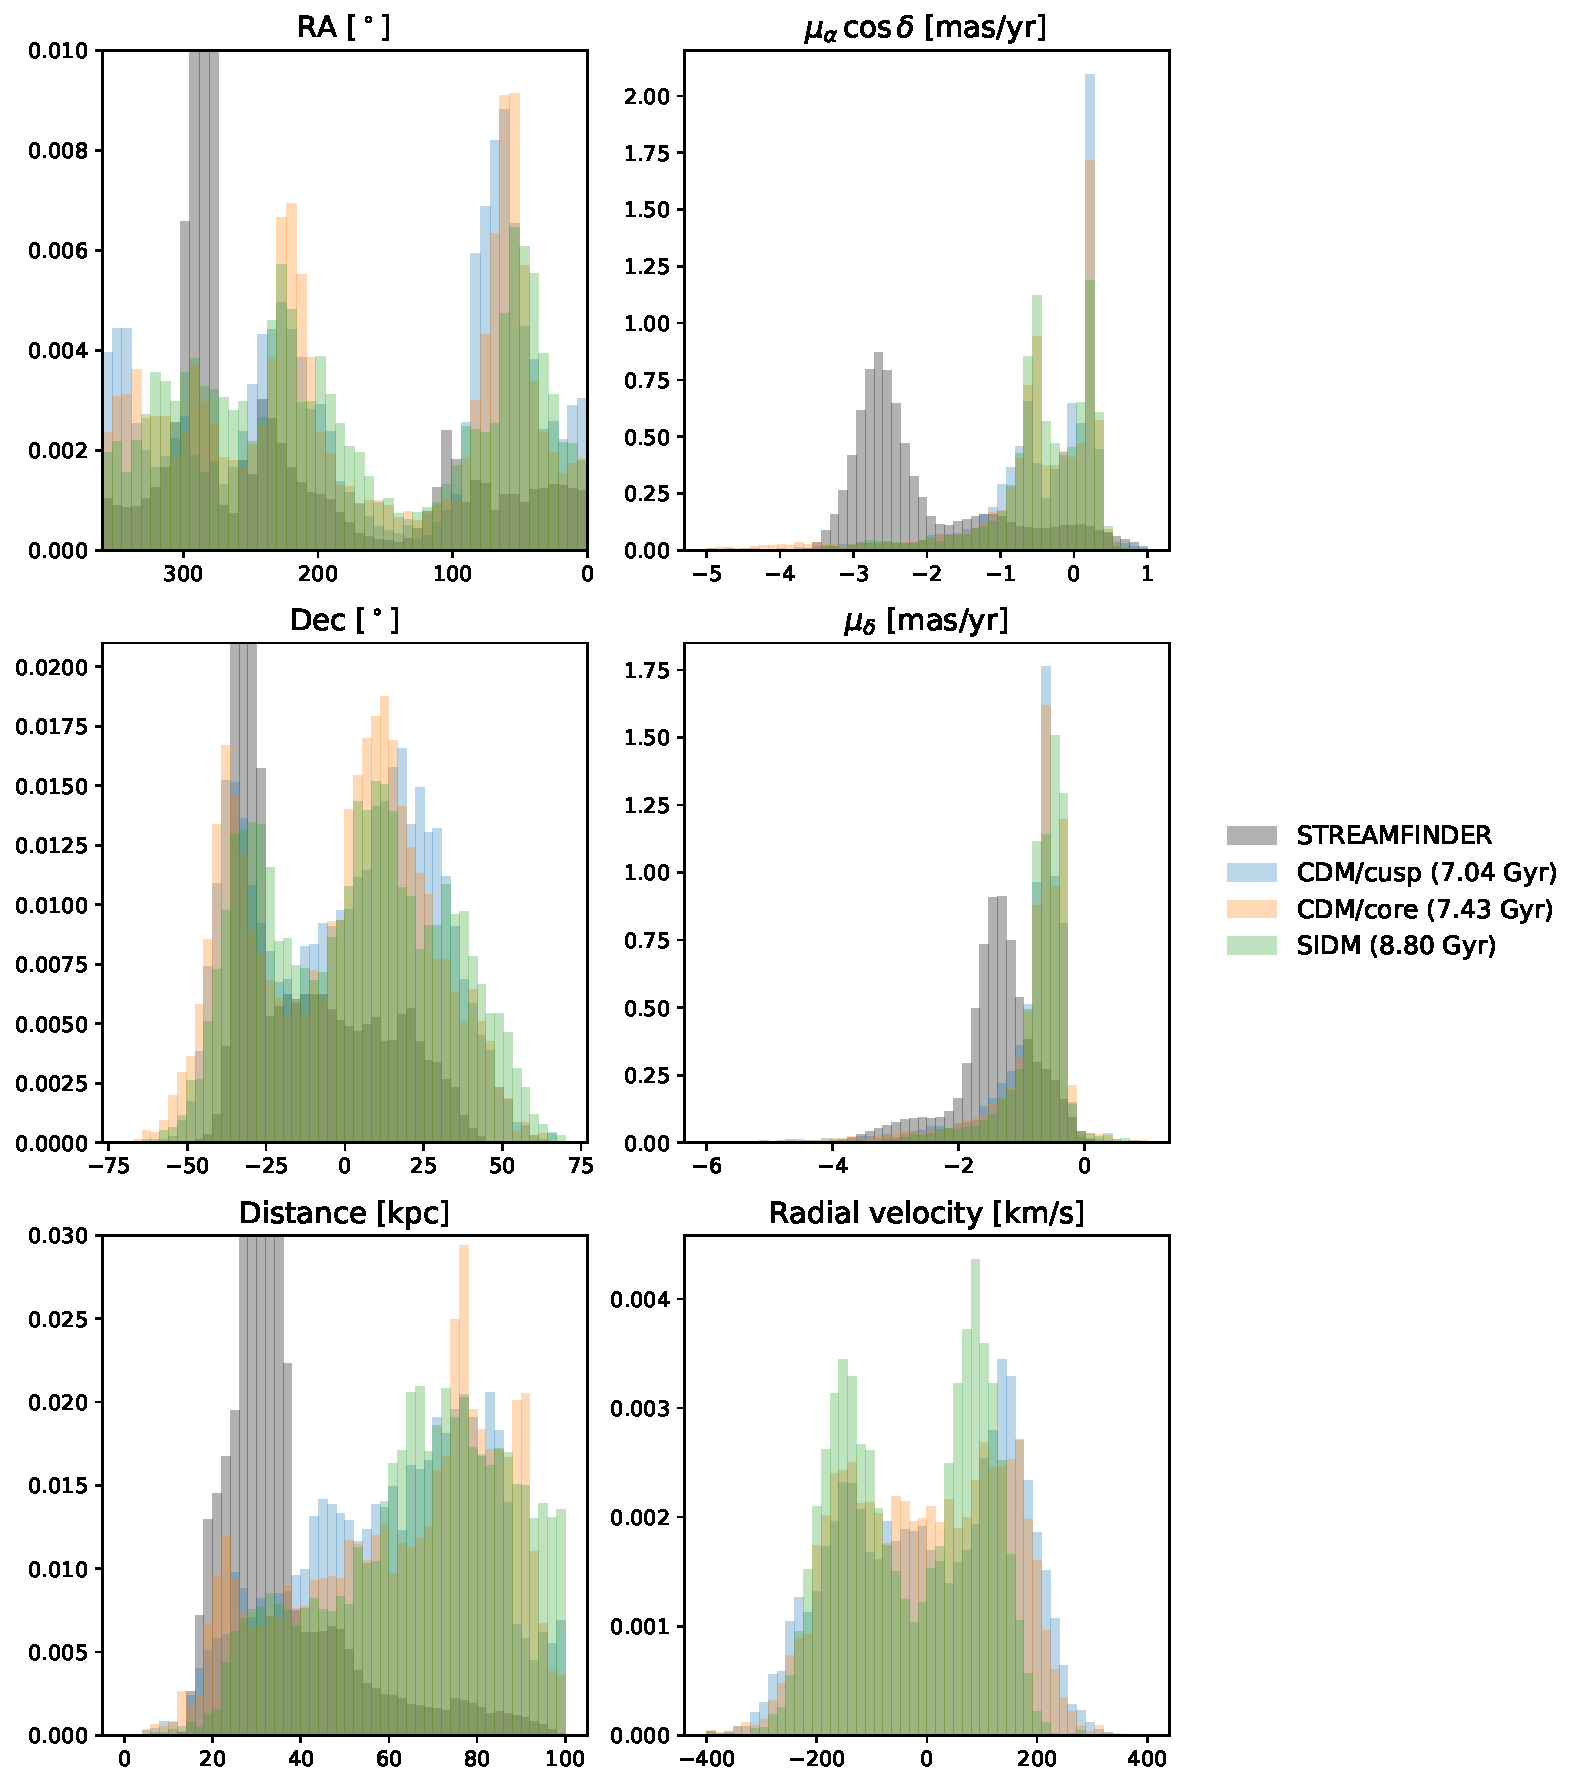
\includegraphics[width=0.9\linewidth]{figs/equatorial_hists.pdf}
%     \caption{%
%         Histograms of the equatorial coordinates and proper motions of the
%         simulated stellar particles closer than 100 kpc and the reference
%         \texttt{STREAMFINDER} stars (where possible).  Note that the
%         \texttt{STREAMFINDER} sample contains a very dense region which is
%         intentionally cut off in the right ascension, declination, and
%         distance plots in order to better see the simulated distributions.
%         All distributions are normalized to unity.
%     }
%     \label{fig:eq_hists}
% \end{figure}

% The histograms show us that the distributions of simulated stars are quite
% different than the \verb|STREAMFINDER| sample, particularly when we consider
% the proper motions and distances. Specifically, the $\mu_\alpha \cos\delta$
% distribution is largely concentrated between $-1$ and $0.5$ mas/yr for all
% three mergers, but appears to be a roughly unimodal distribution at $-2.5$
% mas/yr in the \verb|STREAMFINDER| data.  Similarly, all three mergers show a
% strong peak in $\mu_\delta$ at approximately $-0.5$ mas/yr, compared to the
% strong peak at $-1.5$ mas/yr in the \verb|STREAMFINDER| set. In the distance
% distribution, we see the distribution of distances appear to rise until around
% 60 to 80 kpc, compared to the sharp peak around 30 kpc in the
% \verb|STREAMFINDER| set with a decreasing frequency for larger distances.

% The declination plot shows the existence of peaks around $-30^\circ$ to
% $-40^\circ$ for all mergers and the \verb|STREAMFINDER| set. However, the
% mergers \textit{also} have a peak at around $+20^\circ$ that appears to be
% largely non-existent in \verb|STREAMFINDER|.  Lastly, we note that the right
% ascension plot shows some similarities between all mergers and the
% \verb|STREAMFINDER|: particularly, a peak at around $225^\circ$ and a trough
% at around $140^\circ$.

% The histograms also allow us to highlight some differences between the mergers
% themselves. In particular, the radial velocity histogram confirms the previously
% noted trend. The CDM/cusp merger appears to have more particles with higher
% radial velocity magnitudes than either of the other runs. The CDM/core merger
% appears to have a much flatter distribution of radial velocities than either of
% the other two mergers. The SIDM merger, on the other hand, has a strongly
% bimodal distribution of radial velocities, with strong peaks around $+100$ and
% $-150$ km/s.

